%----------------------------------------------------------------------------------------
%	PACKAGES AND OTHER DOCUMENT CONFIGURATIONS
%----------------------------------------------------------------------------------------

\documentclass{article}

%%%%%%%%%%%%%%%%%%%%%%%%%%%%%%%%%%%%%%%%%
% Lachaise Assignment
% Structure Specification File
% Version 1.0 (26/6/2018)
%
% This template originates from:
% http://www.LaTeXTemplates.com
%
% Authors:
% Marion Lachaise & François Févotte
% Vel (vel@LaTeXTemplates.com)
%
% License:
% CC BY-NC-SA 3.0 (http://creativecommons.org/licenses/by-nc-sa/3.0/)
% 
%%%%%%%%%%%%%%%%%%%%%%%%%%%%%%%%%%%%%%%%%

%----------------------------------------------------------------------------------------
%	PACKAGES AND OTHER DOCUMENT CONFIGURATIONS
%----------------------------------------------------------------------------------------

\usepackage{amsmath,amsfonts,stmaryrd,amssymb} % Math packages

\usepackage{enumerate} % Custom item numbers for enumerations

\usepackage[ruled]{algorithm2e} % Algorithms

\usepackage[framemethod=tikz]{mdframed} % Allows defining custom boxed/framed environments

\usepackage{listings} % File listings, with syntax highlighting
\lstset{
	basicstyle=\ttfamily, % Typeset listings in monospace font
}

%----------------------------------------------------------------------------------------
%	DOCUMENT MARGINS
%----------------------------------------------------------------------------------------

\usepackage{geometry} % Required for adjusting page dimensions and margins

\geometry{
	paper=a4paper, % Paper size, change to letterpaper for US letter size
	top=2.5cm, % Top margin
	bottom=3cm, % Bottom margin
	left=2.5cm, % Left margin
	right=2.5cm, % Right margin
	headheight=14pt, % Header height
	footskip=1.5cm, % Space from the bottom margin to the baseline of the footer
	headsep=1.2cm, % Space from the top margin to the baseline of the header
	%showframe, % Uncomment to show how the type block is set on the page
}

%----------------------------------------------------------------------------------------
%	FONTS
%----------------------------------------------------------------------------------------

\usepackage[utf8]{inputenc} % Required for inputting international characters
\usepackage[T1]{fontenc} % Output font encoding for international characters

\usepackage{XCharter} % Use the XCharter fonts

%----------------------------------------------------------------------------------------
%	COMMAND LINE ENVIRONMENT
%----------------------------------------------------------------------------------------

% Usage:
% \begin{commandline}
%	\begin{verbatim}
%		$ ls
%		
%		Applications	Desktop	...
%	\end{verbatim}
% \end{commandline}

\mdfdefinestyle{commandline}{
	leftmargin=10pt,
	rightmargin=10pt,
	innerleftmargin=15pt,
	middlelinecolor=black!50!white,
	middlelinewidth=2pt,
	frametitlerule=false,
	backgroundcolor=black!5!white,
	frametitle={Command Line},
	frametitlefont={\normalfont\sffamily\color{white}\hspace{-1em}},
	frametitlebackgroundcolor=black!50!white,
	nobreak,
}

% Define a custom environment for command-line snapshots
\newenvironment{commandline}{
	\medskip
	\begin{mdframed}[style=commandline]
}{
	\end{mdframed}
	\medskip
}

%----------------------------------------------------------------------------------------
%	FILE CONTENTS ENVIRONMENT
%----------------------------------------------------------------------------------------

% Usage:
% \begin{file}[optional filename, defaults to "File"]
%	File contents, for example, with a listings environment
% \end{file}

\mdfdefinestyle{file}{
	innertopmargin=1.6\baselineskip,
	innerbottommargin=0.8\baselineskip,
	topline=false, bottomline=false,
	leftline=false, rightline=false,
	leftmargin=2cm,
	rightmargin=2cm,
	singleextra={%
		\draw[fill=black!10!white](P)++(0,-1.2em)rectangle(P-|O);
		\node[anchor=north west]
		at(P-|O){\ttfamily\mdfilename};
		%
		\def\l{3em}
		\draw(O-|P)++(-\l,0)--++(\l,\l)--(P)--(P-|O)--(O)--cycle;
		\draw(O-|P)++(-\l,0)--++(0,\l)--++(\l,0);
	},
	nobreak,
}

% Define a custom environment for file contents
\newenvironment{file}[1][File]{ % Set the default filename to "File"
	\medskip
	\newcommand{\mdfilename}{#1}
	\begin{mdframed}[style=file]
}{
	\end{mdframed}
	\medskip
}

%----------------------------------------------------------------------------------------
%	NUMBERED QUESTIONS ENVIRONMENT
%----------------------------------------------------------------------------------------

% Usage:
% \begin{question}[optional title]
%	Question contents
% \end{question}

\mdfdefinestyle{question}{
	innertopmargin=1.2\baselineskip,
	innerbottommargin=0.8\baselineskip,
	roundcorner=5pt,
	nobreak,
	singleextra={%
		\draw(P-|O)node[xshift=1em,anchor=west,fill=white,draw,rounded corners=5pt]{%
		Question \theQuestion\questionTitle};
	},
}

\newcounter{Question} % Stores the current question number that gets iterated with each new question

% Define a custom environment for numbered questions
\newenvironment{question}[1][\unskip]{
	\bigskip
	\stepcounter{Question}
	\newcommand{\questionTitle}{~#1}
	\begin{mdframed}[style=question]
}{
	\end{mdframed}
	\medskip
}

%----------------------------------------------------------------------------------------
%	WARNING TEXT ENVIRONMENT
%----------------------------------------------------------------------------------------

% Usage:
% \begin{warn}[optional title, defaults to "Warning:"]
%	Contents
% \end{warn}

\mdfdefinestyle{warning}{
	topline=false, bottomline=false,
	leftline=false, rightline=false,
	nobreak,
	singleextra={%
		\draw(P-|O)++(-0.5em,0)node(tmp1){};
		\draw(P-|O)++(0.5em,0)node(tmp2){};
		\fill[black,rotate around={45:(P-|O)}](tmp1)rectangle(tmp2);
		\node at(P-|O){\color{white}\scriptsize\bf !};
		\draw[very thick](P-|O)++(0,-1em)--(O);%--(O-|P);
	}
}

% Define a custom environment for warning text
\newenvironment{warn}[1][Warning:]{ % Set the default warning to "Warning:"
	\medskip
	\begin{mdframed}[style=warning]
		\noindent{\textbf{#1}}
}{
	\end{mdframed}
}

%----------------------------------------------------------------------------------------
%	INFORMATION ENVIRONMENT
%----------------------------------------------------------------------------------------

% Usage:
% \begin{info}[optional title, defaults to "Info:"]
% 	contents
% 	\end{info}

\mdfdefinestyle{info}{%
	topline=false, bottomline=false,
	leftline=false, rightline=false,
	nobreak,
	singleextra={%
		\fill[black](P-|O)circle[radius=0.4em];
		\node at(P-|O){\color{white}\scriptsize\bf i};
		\draw[very thick](P-|O)++(0,-0.8em)--(O);%--(O-|P);
	}
}

% Define a custom environment for information
\newenvironment{info}[1][Info:]{ % Set the default title to "Info:"
	\medskip
	\begin{mdframed}[style=info]
		\noindent{\textbf{#1}}
}{
	\end{mdframed}
}
 % Include the file specifying the document structure and custom commands
\usepackage{bm}
\usepackage{graphicx}
\usepackage[framed,numbered]{mcode}
\usepackage{float}
\usepackage{booktabs}
\graphicspath{{figures/}{}}

%----------------------------------------------------------------------------------------
%	ASSIGNMENT INFORMATION
%----------------------------------------------------------------------------------------

\title{Report of Project-3} % Title of the assignment

\author{Yilang Zhang 16307130242} % Author name and email address

\date{\today} % University, school and/or department name(s) and a date

%----------------------------------------------------------------------------------------

\begin{document}
	
\maketitle % Print the title

%----------------------------------------------------------------------------------------
%	PROBLEM 1
%----------------------------------------------------------------------------------------

\section{Neural Network} % Numbered section

To start with, I used the provided code to train a model and predict on both training and validation set. Then I modified it to visualize the training process. The change of MSE during training are shown in \textbf{Figure \ref{fig1}} and train and validation error are shown in command line below.

\begin{figure}[H]
	\centering
	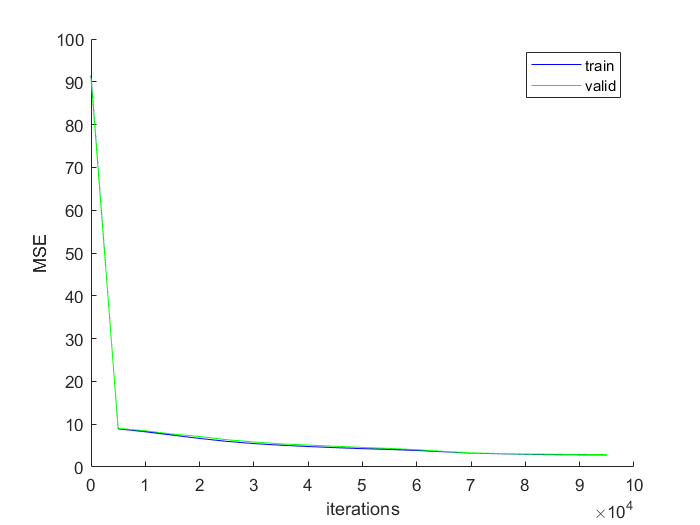
\includegraphics[scale=0.5]{figure1}
	\caption{The training process of the provided code.}
	\label{fig1}
\end{figure}

\begin{commandline}
	\begin{verbatim}
	Training iteration = 0, train error = 0.9054, validation error = 0.9064
	Training iteration = 5000, train error = 0.6086, validation error = 0.6198
	...
	Training iteration = 90000, train error = 0.4522, validation error = 0.4778
	Training iteration = 95000, train error = 0.4446, validation error = 0.4708
	\end{verbatim}
\end{commandline}

After iterations for $10^5$ times, mean square error converge on both training and validation set,but the model could only achieve an error rate of $47.08\%$ on the validation set, which implies that the freedom of parameters in the model is far not enough, i.e. the model is too simple to cover such a classification over 10 classes. Next, I'll improve the performance of the model by adjust its structure and parameters in order to increase the complexity of the model.

%------------------------------------------------

\subsection{Network structure}

In this part, I try to change the number of nodes (neurons) in each hidden layer and the depth of the model perspectively. In order to speed up the training process, I reduce the number of iterations to $10^4$ and compare across the changes.

\begin{figure}[H]
	\centering
	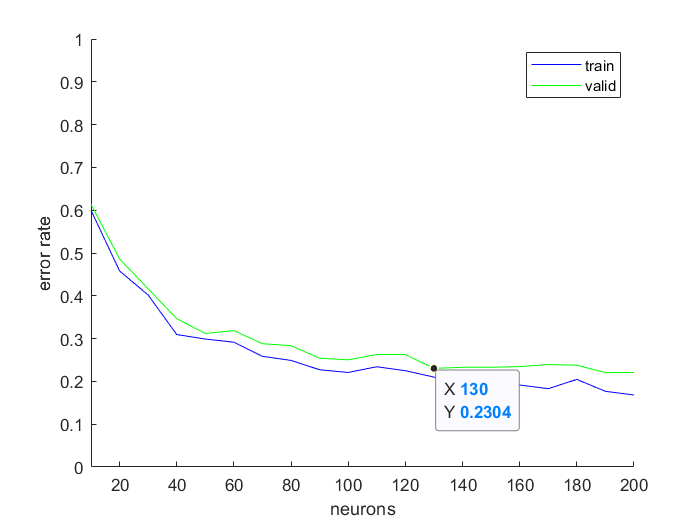
\includegraphics[scale=0.5]{figure2}
	\caption{Experiment on the number of neurons in the first layer.}
	\label{fig2}
\end{figure}

In \textbf{Figure \ref{fig2}}, I keep the number of hidden layer in the model (the depth) to be 1 and change the number of neurons in the first hidden layer ranging from 10 to 200, step by 10. And from the figure we can see that the error rate on the validation set converge approximately when the number of neurons increase to 130, and change slightly with the increasing of it after 130. So I choose 130 as the best number of neurons in the first hidden layer.

\begin{figure}[H]
	\centering
	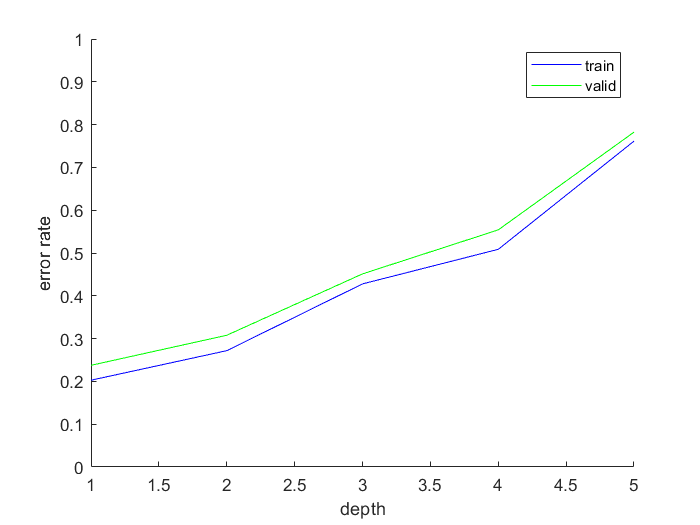
\includegraphics[scale=0.5]{figure3}
	\caption{Experiment on the depth (the number of hidden layers) of the model.}
	\label{fig3}
\end{figure}

In \textbf{Figure \ref{fig3}}, I increase the depth of the model while keeping the neurons in each layer being 130. But the results are surprising that the error rate goes high when the model gets deeper. I suspect that the neurons needed in other hidden layers may be different from the first layer, so I experiment with different numbers of neurons in other layers, but the results didn't change. All the error rates of multiple-layer models are higher than single layer.

In fact, with the increasing of depth, the model becomes more complex very rapidly, making it harder to convergence. And 1 layer is sufficient to cover this classification problem. Finally, I choose the structure of 1 layer with 130. It's performance (with $10^5$ iterations of training) are shown below, which is much better than the initial version.

\begin{commandline}
	\begin{verbatim}
	train error = 0.1934, validation error = 0.2238
	\end{verbatim}
\end{commandline}

\subsection{Training procedure}

In the second part, there are two factors should be taken into consideration: the learning rate and the momentum strength. In my codes, I use a variable $w\_pre$ to store last weights and perform
\[
w^{t+1}=w^t-\alpha_t\nabla f(w^t)+\beta_t(w^t-w^{t-1})
\]
with learning rate ranging from $10^{-5}$ to $10^{-1}$, step by $10^{-1}$ and run 10 times to get the average. We can infer from \textbf{Figure \ref{fig4}} that $\alpha_t=10^{-4}$ is the best learning rate which has the lowest error rate on training and validation set.

\begin{figure}[H]
	\centering
	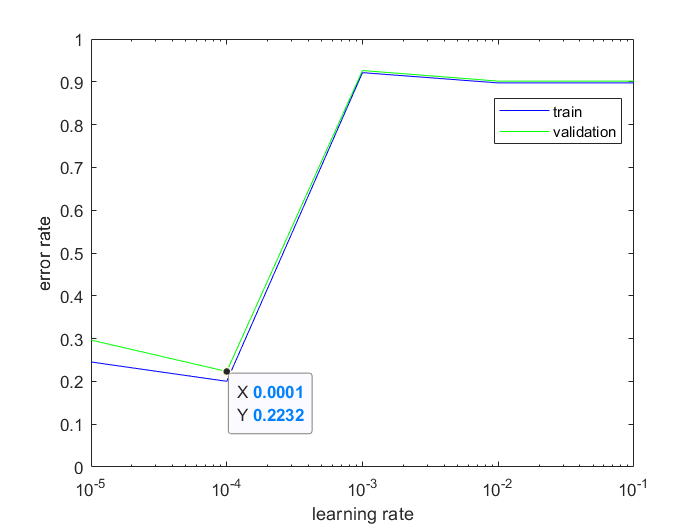
\includegraphics[scale=0.5]{figure4}
	\caption{Experiment with learning rate.}
	\label{fig4}
\end{figure}

\begin{commandline}
	\begin{verbatim}
	train error = 0.2000, validation error = 0.2232
	\end{verbatim}
\end{commandline}

It seems that the momentum has no significant effect on our model, but in fact it accelerate training procedure, especially the speed of convergence remarkably. In our model, we use a common learning for all of our parameters, but it may not be suitable for all the dimension and all the hidden layers. This brings about a problem that some dimensions have small gradients and some with enormous ones. The dimensions with small gradients will converge slowly, during which the dimensions with enormous gradients will 'jump' drastically and can hardly reaches the primal point.\par
Momentum act as a buffer for these huge gradients, contracting with the drastic change of huge gradients. When $w^t$ changes drastically, the term $\beta_t(w^t-w^{t-1})$ will be huge and restrain excessive descending along the gradient, while the term will be small enough to be omitted when $w^t$ changes at a moderate speed. Although with more parameters (130), the model which includes a momentum term during SGD converges quickly.

\subsection{Vectorized evaluation}

In this part, I use fully vectorized matrix computation to substitute for-loops in initial code. I'll deduct the matrix form of forward and backpropagation:\par

Consider a model with $h-1$ hidden layers, which are listed in \textbf{Table \ref{tab1}}.

\begin{table}[H]
	\centering
	\caption{Notation and size for matrices.}
	\label{tab1}
	\begin{tabular}{cccccc}
	\toprule
	Input $X$& Input weights $W_i$& Hidden layer 1 $W_1$& $\dots$ &Output weights $W_o$& Output $\hat{y}$\\
	\midrule
	$d\times{n_i}$& $n_i\times{n_1}$& $n_1\times{n_2}$& $\dots$& $n_h\times{n_o}$& $n_o\times{c}$\\
	\bottomrule
	\end{tabular}
\end{table}

\paragraph{Forward evaluation}
Multiply the matrices one by one. Use $IP$ and $FP$ to store the value of intermediate weights.
\[
\begin{aligned}
IP_1&=X\times W_i\\
FP_j&=tanh(IP_j),  1\le{j}\le{h}\\
IP_k&=FP_{k-1}\times W_{k-1},  2\le{k}\le{h}\\
\hat{y}&=FP_{h}\times W_o\\
L&=\|y-\hat{y}\|_2^2
\end{aligned}
\]

\paragraph{Backpropagation}
Owing to the fact that we use squared error $L$ as our loss function, we have:
\[
\begin{aligned}
\frac{\partial L}{\partial W_0}
&=\frac{\partial \hat{y}}{\partial W_o}\frac{\partial L}{\partial \hat{y}}\\
&=FP^T_h\times 2(\hat{y}-y)\\
\frac{\partial{L}}{\partial{IP_{h-1}}}
&=\frac{\partial{FP_{h-1}}}{\partial{IP_{h-1}}}\frac{\partial{L}}{\partial{FP_{h-1}}}\\
&=sech(IP_{h-1})\cdot sech(IP_{h-1})\cdot(2(\hat{y}-y)\times W_o^T)\\
\frac{\partial{IP_j}}{\partial{IP_{j-1}}}
&=\frac{\partial{FP_{j-1}}}{\partial{IP_{j-1}}}\frac{\partial{IP_j}}{\partial{FP_{j-1}}}\\
&=sech(IP_{j-1}) \cdot sech(IP_{j-1})\cdot W_{j-1}\\
\frac{\partial{IP_j}}{\partial{W_{j-1}}}
&=FP_{k-1}\\
\frac{\partial IP_i}{\partial W_i}
&=X^T\\
\end{aligned}
\]

where '$\times$' represents for cross-product and '$\cdot$' represents for dot-product.

Then use chain rule and we can get any $\frac{\partial{L}}{\partial{W_j}},j=i,1,\dots,h-1,o$. Corresponding core codes are shown as follows:

\begin{lstlisting}
% Compute Output (fully vectorized)
ip{1} = X * inputWeights;
fp{1} = tanh(ip{1});
for h = 2:length(nHidden)
    ip{h} = fp{h-1} * hiddenWeights{h-1};
    fp{h} = tanh(ip{h});
end
yhat = fp{end} * outputWeights;

relativeErr = yhat - y;
f = relativeErr(:)' * relativeErr(:);

if nargout > 1
    err = 2 * relativeErr;
    
    % Output Weights
    gOutput = fp{end}' * err;
    
    if length(nHidden) > 1
        % Last Layer of Hidden Weights
        clear backprop
        backprop = err * outputWeights' .* (sech(ip{end}).^2);
        
        % Other Hidden Layers
        for h = length(nHidden)-2:-1:1
            backprop = backprop * hiddenWeights{h+1}' .* (sech(ip{h+1}).^2);
            gHidden{h} = fp{h}' * backprop;
        end
        
        % Input Weights
        backprop = backprop * hiddenWeights{1}' .* (sech(ip{1}).^2);
        gInput = X' * backprop;
    else
        % Input Weights
        gInput = X' * err * outputWeights' .* (sech(ip{end}).^2);
    end
end
\end{lstlisting}
 
After replacing for-loops with fully-vectorized matrix operations in functions $MLPclassificationLoss.m$ and $MLPclassificationPredict.m$, the speed of training increased overwhelmingly!
 
\subsection{Weight decay}

In this part, I choose to use $l_2$ regularization. The loss function becomes $E=L+\frac{\lambda}{2}\|W\|_2^2$ and gradient $\frac{\partial E}{\partial W}=\frac{\partial L}{\partial W}+\lambda W$, where $\lambda$ is a hyperparameter.\par


\begin{figure}[H]
	\centering
	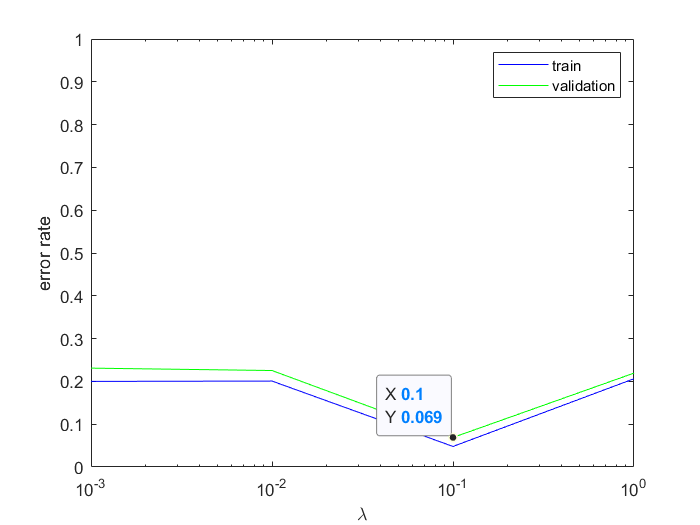
\includegraphics[scale=0.5]{figure5}
	\caption{Experiment with $l_2$ regularization coefficient $\lambda$.}
	\label{fig5}
\end{figure}

I experiment with $\lambda$ from $10^{-3}$ to $10^{0}$, results are shown in \textbf{Figure \ref{fig5}}. $\lambda=10^{-1}$ has the lowest error rate on validation set, I choose it as the coefficients for $l_2$ regularization, thus reaching an error rate of $6.90\%$ on validation set.

\begin{info}[Notice]
It should be stressed that the biases shouldn't be punished, as it only controls the height of the function but not its complexity.
\end{info}

\begin{lstlisting}
% Exclude bias when regularizing
w(~bias) = w(~bias) - learningRate * lambda * w(~bias);
\end{lstlisting}


\subsection{Softmax}

In this part, output $\hat{y}$ has been put into a softmax layer, converting to the probabilities $p(y_i)$ of each class, then I replace squared error with the negative log-likelihood of the true label under softmax loss. Forward evaluation and backpropagation are modified to fit in with the new output and loss function.

\paragraph{Forward evaluation}
We still use the equations and procedure in \textbf{1.3} except for the function of $L$. Added parts and modified parts are listed below.

\[
\begin{aligned}
p(y_i)&=\frac{exp(y_i)}{\sum_{j=1}^cexp(y_j)}\\
L&=-\ln p(y_i)
\end{aligned}
\]

\paragraph{Backpropagation}
In \textbf{1.3} we use $\frac{\partial L}{\partial \hat{y}}=2(\hat{y}-y)$ as the derivative of $L$ sub $\hat{y}$. Here we only change this equation while reserving other parts of backpropagation. 
\[
\begin{aligned}
\frac{\partial L}{\partial p(y_i)}&=-\frac{1}{p(y_i)}\\
\frac{\partial p(y_i)}{\partial \hat{y_i}}&=
\begin{cases}
p(y_i)(1-p(y_i))& i=j\\
-p(y_i)p(y_j) & i\neq j
\end{cases}
\\
\frac{\partial L}{\partial \hat{y_i}}&=\frac{\partial L}{\partial p(y_i)}\frac{\partial p(y_i)}{\partial \hat{y_i}}\\
&=
\begin{cases}
p(y_i)-1& i=j\\
p(y_j) & i\neq j
\end{cases}
\end{aligned}
\]

Modified parts of core codes are shown beneath (see full codes in $MLPclassificationLoss.m$). A small trick has been used here when computing the softmax score of the outputs: In each instance, I shift all the value of $\hat{y_i}$ by $-\max_j(\hat{y_j})$ to avert overflow when evaluating $exp(y_i)$, therefore both the numerator and denominator of $p(y_i)$ are multiplied by $\exp(-\max_j(\hat{y_j}))$, so $p(y_i)$ won't change.

\begin{lstlisting}
% Compute Output (fully vectorized)
ip{1} = X * inputWeights;
fp{1} = tanh(ip{1});
for h = 2:length(nHidden)
    ip{h} = fp{h-1} * hiddenWeights{h-1};
    fp{h} = tanh(ip{h});
end
yhat = fp{end} * outputWeights;

% Softmax layer
yhat_shift_exp = exp(yhat - max(yhat,[],2));
denom = sum(yhat_shift_exp,2) * ones(1,nLabels);
py = yhat_shift_exp ./ denom;

% Negative log-likelihood of the true label
index = (y == 1);
f = sum(-log(py(index)));
err = py;
err(index) = py(index) - 1;
\end{lstlisting}

After altering the output layer and loss function, other hyperparameters including the structure of network, learning rate $\alpha_t$, regularization parameter $\lambda$ and number of iterations. Repeat experiments which has been done in previous parts, we get new hyperparameters in \textbf{Table \ref{tab2}}.

\begin{table}[H]
	\centering
	\caption{New hyperparameters attained from experiments.}
	\label{tab2}
	\begin{tabular}{ccccc}
	\toprule
	depth $h$& neurons& learning rate $\alpha_t$& regularization strength $\lambda$ &iterations\\
	\midrule
	1& 130& $10^{-3}$& $10^{-2}$& $10^5$\\
	\bottomrule
	\end{tabular}
\end{table}

Run for 10 times and an average validation error of $6.58\%$ has been achieved. The model has been improved a little.

\begin{figure}[H]
	\centering
	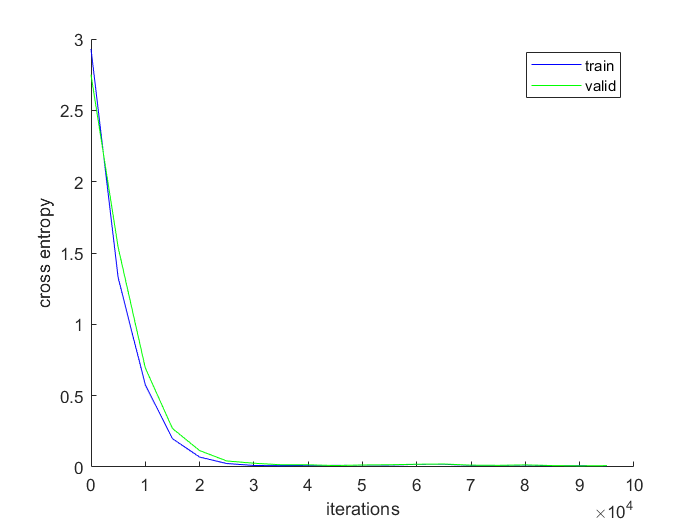
\includegraphics[scale=0.5]{figure6}
	\caption{Model with softmax layer and cross entropy loss function.}
	\label{fig6}
\end{figure}

\begin{commandline}
	\begin{verbatim}
	train error = 0.0374, validation error = 0.0658
	\end{verbatim}
\end{commandline}

\subsection{Bias}

In this part, a bias has been added to each layer through complicated modification.

\paragraph{1}
The number of parameters should be changed by adding a row to the bottom of each matrix.

\begin{lstlisting}
nParams = d * nHidden(1);
for h = 2:length(nHidden)
    % add a bias for each layer
    nParams = nParams + (nHidden(h-1) + 1) * nHidden(h);
end
nParams = nParams + (nHidden(end) + 1) * nLabels;
w = randn(nParams,1);
\end{lstlisting}

\paragraph{2}
When implementing BP algorithm: In forward evaluation, a column filled with $1$ should be added to the right of the output matrix in each hidden layer. In backpropagation, this column should be removed to fit the shape of matrix in previous layer in order to execute matrix multiplication. Related codes are shown below.

\begin{lstlisting}
% Form Weights
offset = nVars*nHidden(1);
inputWeights = reshape(w(1:offset),nVars,nHidden(1));
for h = 2:length(nHidden)
    % The last row filled with bias
    hiddenWeights{h-1} = reshape(w(offset+1:offset+(nHidden(h-1)+1)*nHidden(h)),...
        nHidden(h-1)+1,nHidden(h));
    offset = offset + (nHidden(h-1) + 1) * nHidden(h);
end
outputWeights = w(offset+1:offset+(nHidden(end)+1)*nLabels);
outputWeights = reshape(outputWeights,nHidden(end)+1,nLabels);

% Compute Output (fully vectorized)
% Add bias
ip{1} = [X * inputWeights,zeros(nInstances,1)]; % Add zeros just for convenience
fp{1} = tanh(ip{1});
fp{1}(:,end) = 1;
for h = 2:length(nHidden)
    % Add bias
    ip{h} = [fp{h-1} * hiddenWeights{h-1},zeros(nInstances,1)];
    fp{h} = tanh(ip{h});
    fp{h}(:,end) = 1;
end
yhat = fp{end} * outputWeights;

% Softmax layer
yhat_shift_exp = exp(yhat - max(yhat,[],2));
denom = sum(yhat_shift_exp,2) * ones(1,nLabels);
py = yhat_shift_exp ./ denom;

% Negative log-likelihood of the true label
index = (y == 1);
f = sum(-log(py(index)));
err = py;
err(index) = py(index) - 1;

if nargout > 1
    
    % Output Weights
    gOutput = fp{end}' * err;
    
    if length(nHidden) > 1
        % Last Layer of Hidden Weights
        clear backprop
        backprop = err * outputWeights' .* (sech(ip{end}).^2);
        backprop = backprop(:,1:end-1); % Remove extra column used for bias
        
        % Other Hidden Layers
        for h = length(nHidden)-2:-1:1
            backprop = backprop * hiddenWeights{h+1}' .* (sech(ip{h+1}).^2);    
            backprop = backprop(:,1:end-1); % Remove extra column used for bias
            gHidden{h} = fp{h}' * backprop;
        end
        
        % Input Weights
        backprop = backprop * hiddenWeights{1}' .* (sech(ip{1}).^2);
        backprop = backprop(:,1:end-1); % Remove extra column used for bias
        gInput = X' * backprop;
    else
        % Input Weights
        gInput = X' * err * outputWeights' .* (sech(ip{end}).^2);
        gInput = gInput(:,1:end-1);  % Remove extra column used for bias
    end
end
\end{lstlisting}

\paragraph{3}
After adding a bias for each layer, we should exclude bias from our regularization, as said in \textbf{1.4}, it only controls the height of the function but not its complexity. So I modified the function $MLPclassificationLoss$ to  return an additional boolean vector $bias$ which marks the position of bias in weight vector $w$. Thus We can only penalize the weights and not the bias term.

\begin{lstlisting}
i = ceil(rand*num_train);
[f,g,bias] = funObj(w,i);
w_pre = w;
% Exclude bias when regularizing
w = w - stepSize * g - momentum * (w - w_pre);
w(~bias) = w(~bias) - lambda * w(~bias);
\end{lstlisting}

\paragraph{Results and analysis}
Adding a bias the each layer of our model didn't have a palpable effect on it. Running for 10 times, we attain an average validation error of $10.82\%$, which is not distinctly different from the results in \textbf{1.5}.\par

\begin{commandline}
	\begin{verbatim}
	train error = 0.0302, validation error = 0.0598
	\end{verbatim}
\end{commandline}

This phenomenon doesn't goes beyond my expectation. Notice that there is only one hidden layer in the model, so this part of work has only added $10$ bias to our model, which seems a minute change compared with the number of total parameters ($8020$). So the model has just improved a little ($\%0.06$), but it's enough.

\subsection{Dropout}

Random dropout the weights with $p=0.5$ when training and multiply the weights with $p=0.5$ beforehand when predicting (Notice that $E(w)=1\times pw+0\times (1-p)w=0.5w$), finally the model reaches a validation error rate of $15.26\%$, which is a little worse than the results in preceding parts.

\begin{commandline}
	\begin{verbatim}
	train error = 0.0652, validation error = 0.0760
	\end{verbatim}
\end{commandline}

Dropout play as a role to avoid overfitting. One explanation is that abandon some units and edges randomly actually a kind of pattern selection. Another explanation interpret it as an approach of random combination of networks with different structure. That is to say, for a model with $n$ nodes, random dropout generates $\binom{n}{1}+\binom{n}{2}+\dots+\binom{n}{n}=2^n$ different models and combine them with different probabilities.\par
But the results shows that dropout didn't come into effect as we wish. This is because there are not so much nodes and edges in our model, and we haven't meet up with an obvious risk of overfitting. In other words, the model is not deep enough to implement dropout. However, we can't deny that dropout could have a good performance in deep networks.\par
Based on above discussion, I decide to exclude dropout in the model.

\subsection{Fine-tuning of the last layer}

In earlier courses, we learned that for a linear regression problem with squared loss,
\[
\begin{aligned}
\min L=\|y-\hat{y}\|_2^2 \\
s.t.\quad XW=y
\end{aligned}
\]
it has a close-form solution, the least square solution $W=X^{\dag}y=(X^TX)^{-1}y$ and $\hat{y}=XW=X(X^TX)^{-1}y$.\par
But under the circumstance of a cross-entropy loss,
\[
\begin{aligned}
L=\sum_n-\ln p(\hat{y}_i^{(n)})\\
s.t.\quad XW=y
\end{aligned}
\]
we can't find a close-form solution for it. And it's uneconomical to change back to squared error for trade of speed, which could in return decline the correct rate of prediction. So here we still use cross-entropy as our error and didn't change the evaluation of the gradient for the output weights.

\subsection{Extend data}

By applying small transformations such as translations, rotations,
resizing and etc., one can get more training examples from the origin data. I applied random translations, rotations and resizing for respectively 1000 samples, expanding the training data to 8000 examples. \par
The shift distance in transformation are generated from normal distribution $N(0,4)$. The angle in rotation are generated from $N(0,25)$. The scale in resizing are are generated from $N(1,0.01)$. The results are shown below.

\begin{commandline}
	\begin{verbatim}
	train error = 0.0623, validation error = 0.0863
	\end{verbatim}
\end{commandline}

In this case, transformation has a bad effect on the model. To explore why transformation has lost efficiency, I choose an image from the training set randomly, enlarge it for 3 times and show it in \textbf{Figure \ref{fig7}}. The image almost occupies the whole space of the image. When it's transformed, even a trivial transformation, could damage significant information it contains. So transformation is not a good idea here to generate extended data and I'll exclude it from my model, but it's a good method for those training set with bigger images.

\begin{figure}[H]
	\centering
	
\includegraphics[scale=3]{figure7}
	\caption{An image randomly selected from training set.}
	\label{fig7}
\end{figure}


\subsection{Convolutional layer}
Related codes for \textbf{1.1$\sim$1.9} are stored in $neuralNetwork.m$, $MLPclassificationLoss.m$ and\\ $MLPclassificationPredict.m$. Three new Matlab files $CNN.m$, $CNNclassificationLoss.m$ and\\ $CNNclassificationPredict.m$ are built for the convolutional part.

\paragraph{Forward evaluation}
In the forward procedure, each instance in input data of size $1\times 256$ are reverted to its origin shape $16\times 16$. Every hidden layer are convoluted with the output of previous layer, and the output of the last layer are stretched into a column then pass through a fully connected layer and a softmax layer to form the probability of each class. Modified equations and core codes are showed below.

\[
\begin{aligned}
IP_1&=X\ast W_1\\
IP_k&=FP_{k-1}\ast W_k
\end{aligned}
\]
where '$\ast$' represents for the convolution operation. And here we use 2-dimensional convolution: $C(j,k)=A(j,k)*B(j,k)=\sum_p\sum_qA(p,q)B(j-p+1,k-q+1)$.



\begin{lstlisting}
% Forward evaluation
ip = cell(h,1);
fp = cell(h,1);
padding = padarray(reshape(X(i,:),width,width)[padsize(1),padsize(1)],0,'both');
ip{1} = conv2(padding,hiddenWeights{1},'valid');
fp{1} = tanh(ip{1});
for h = 2:length(filter)
	padding = padarray(fp{h-1},[padsize(h),padsize(h)],0,'both');
    ip{h} = conv2(padding,hiddenWeights{h},'valid');
    fp{h} = tanh(ip{h});
end
yhat = [fp{end}(:);1]' * outputWeights;
    
% Softmax layer
yhat_shift_exp = exp(yhat - max(yhat,[],2));
denom = sum(yhat_shift_exp,2) * ones(1,nLabels);
py = yhat_shift_exp ./ denom;
    
% Negative log-likelihood of the true label
index = (y == 1);
f = f + sum(-log(py(index)));
err = py;
err(index) = py(index) - 1;
\end{lstlisting}

\paragraph{Backpropagation}
The procedure of backpropagation is intricate, but the TA of the class had told us the approach to evaluate the gradient of the convolutional layer, which are shown in \textbf{Figure \ref{fig8}}. What should be done is mirror transforming the rows and columns of the matrices, i.e. reversing the order of elements in matrices.

\begin{figure}[H]
	\centering
	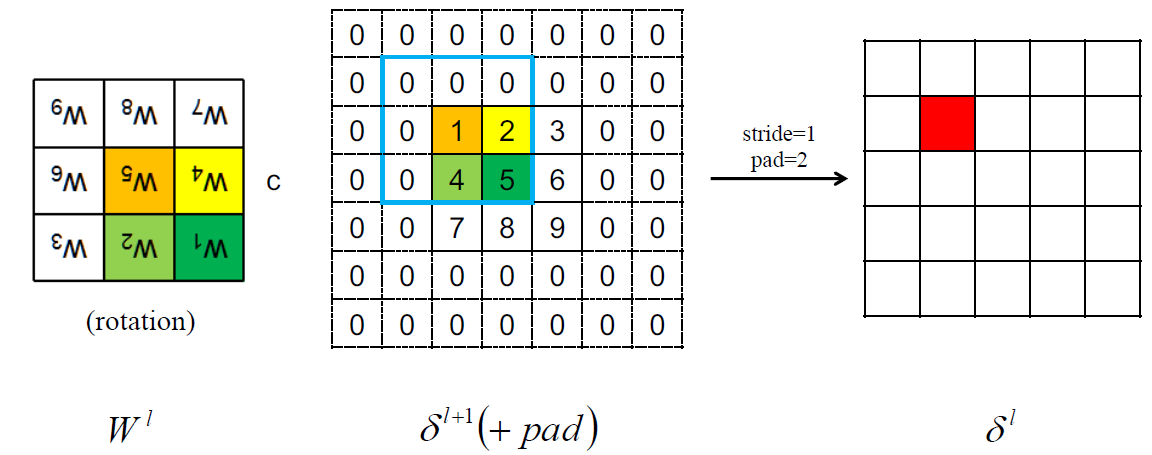
\includegraphics[scale=0.5]{figure8}
	\caption{The procedure to evaluate the gradient of the convolutional layer.}
	\label{fig8}
\end{figure}

Specifically speaking, in our network:
\[
\begin{aligned}
\frac{\partial L}{\partial IP_{k-1}}&=\frac{\partial FP_k}{\partial IP_{k-1}}\frac{\partial L}{\partial FP_k}\\
&=W_k^{rev}\ast\frac{\partial L}{\partial FP_k}\\
\frac{\partial L}{\partial W_k}&=\frac{\partial FP_k}{\partial W_k}\frac{\partial L}{\partial FP_k}\\
&=IP_{k-1}^{rev}\ast\frac{\partial L}{\partial FP_k}\\
\frac{\partial L}{\partial W_1}&=\frac{\partial FP_1}{\partial W_1}\frac{\partial L}{\partial FP_1}\\
&=X^{rev}\ast\frac{\partial L}{\partial FP_k}\\
\end{aligned}
\]
where $A^{rev}$ represents for the reverse rearrangement of matrix A which has been illustrated above.\par
Here are related codes. Notice that we use the $valid$ option of function $conv2$ to get the convolution that are computed without zero-padded edges.

\begin{lstlisting}
% back propagation
% Output Weights
gOutput = gOutput + [fp{end}(:);1] * err;

% Last Layer of Hidden Weights
clear backprop
% Remove extra column used for bias
backprop = reshape(err * outputWeights(1:end-1,:)',size(fp{end}));
backprop = backprop .* (sech(ip{end}).^2);

% Other Hidden Layers
for h = length(filter)-1:-1:1
    gHidden{h+1} = gHidden{h+1} + conv2(fp{h},backprop,'valid');
    backprop = conv2(backprop,ihiddenWeights{h+1}) .* (sech(ip{h}).^2);
end
    
% Input Weights
ix = reshape(X(i,end:-1:1),width,width);
gHidden{1} = gHidden{1} + conv2(ix,backprop,'valid');
\end{lstlisting}

\paragraph{Results and analyse}
By experimenting with all of the hyperparameters which is the same as what have been done in \textbf{1.1 $\sim$ 1.9}. The best hyperparameters are listed in \textbf{Figure \ref{tab3}}.

\begin{table}[H]
	\centering
	\caption{Best hyperparameters chosen by experiments in CNN.}
	\label{tab3}
	\begin{tabular}{ccccccc}
	\toprule
	network depth $h$& filter size $F$& stride $S$& padding $P$& learning rate $lr$& regularization $\lambda$& iterations\\
	\midrule
	1& $3\times 3$& 1& 0& $10^{-3}$& $10^{-2}$& $10^{5}$\\
	\bottomrule
	\end{tabular}
\end{table}

Finally we get a convolutional neural network model with validation error of $8.70\%$. It's higher than the validation error of the model who only utilize fully connected network as the hidden layer, which suggests that this model is worse than it.

\begin{commandline}
	\begin{verbatim}
	train error = 0.0640, validation error = 0.0870
	\end{verbatim}
\end{commandline}

There are some reasons for it and improvements could be done. There are more parameters in a one-layer fully connected model than in a one-layer CNN model because of parameter sharing in covolutional layer. If we want to use more parameters in CNN, we need to deepen the network, but it contradict with the size of the pictures, which is only $16\times 16$ pixels. So the size could becomes so small through several convolutional layers and thus making it difficult to recognize more patterns and information from it. As a simple convolutional layer could only recognize limited patterns of the input data.
Furthermore, there are several other methods of improvement should be taken into consideration, which will also be discussed in the extra parts.


\subsection{Extra part: improvements}
In this part, I tried with some methods that are not on the question list to optimize my model.\par
I tried with multiple kernels in one layer, replacing activation function with $ReLu$, batch normalization, Adam optimization algorithm and mini-batch gradient descent. Through experiments, I found that only the mini-batch gradient descent has improved the model, while others do little with it. Different size of batch are tried, and the one including 10 instances has the best effect.\par
\textbf{BGD} (batch gradient descent) performs training with the whole training set in each iterations, it has several problems:\par
(1) It takes a lot of time perform training, especially when there are numerous instances in the training set.\par
(2) It risks overfitting.\par
\textbf{SGD} (stochastic gradient descent) performs training with only one random instance to overcome the complexity of evaluation in BGD, but it also has some deficiencies:\par
(1) It lacks of accuracy due to the randomness of the instance. Although the objective function is strictly convex, it cannot convergence linearly.\par
(2) It may convergence to local primal, because one instance couldn't represent the whole training set, especially when there are bad instances or outliers.

\textbf{MBGD} (mini-batch gradient descent) seems like a compromise between SGD (stochastic gradient descent) and BGD (batch gradient descent), but it really absorbs the merits of both and overcomes the deficiency of both. It could convergence quickly and linearly with less evaluation complexity than BGD. I performed it on both fully connected neural network and convolutional neural network. The results are showed in the bottom. MBGD improves both the performance of CNN and FCNN and CNN markedly.

\begin{commandline}
	\begin{verbatim}
	FCNN:
	train error = 0.0002, validation error = 0.0382
	CNN:
	train error = 0.0438, validation error = 0.0762
	\end{verbatim}
\end{commandline}

\subsection{Final model and results}
Consequently, I choose fully connected neural network with structure below and hyperparameters in \textbf{Table \ref{tab4}}.
\[
\mathop{X}\limits_{n\times(d+1)}\xrightarrow[(d+1)\times n_1]{W_1}
\mathop{IP_1}\limits_{n\times n_1}\xrightarrow[bias]{tanh}
\mathop{FP_1}\limits_{n\times(n_1+1)}\xrightarrow[(n_1+1)\times c]{W_o}
\mathop{Z}\limits_{n\times c}\xrightarrow{softmax}
\mathop{PY}\limits_{n\times c}\xrightarrow{cross-entropy}
J
\]

\begin{table}[H]
	\centering
	\caption{Hyperparameters in final model.}
	\label{tab4}
	\begin{tabular}{ccccccc}
	\toprule
	depth & neurons $n_1$ & momentum & learning rate $lr$& regularization $\lambda$& iterations & batch size\\
	\midrule
	1 & 130 & 0.9 & $10^{-3}$ & $10^{-2}$ & $10^{5}$ & 10\\
	\bottomrule
	\end{tabular}
\end{table}

Training procedure and results (run for 10 times and compute the average):

\begin{figure}[H]
	\centering
	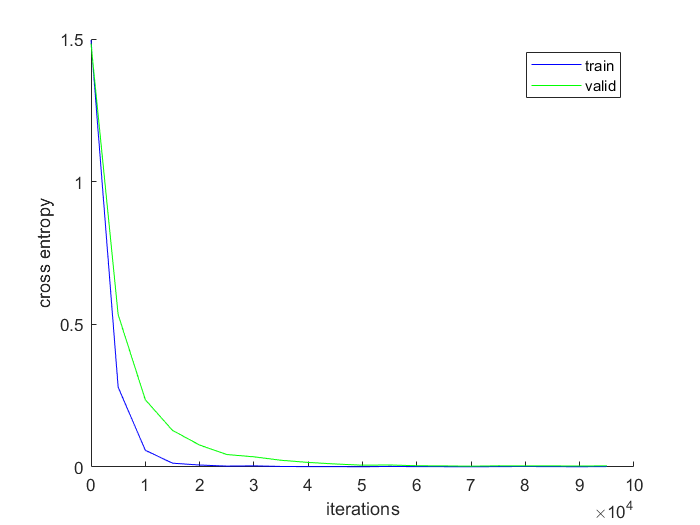
\includegraphics[scale=0.5]{figure9}
	\caption{Change of cross-entropy when training in the final model.}
	\label{fig9}
\end{figure}

\begin{commandline}
	\begin{verbatim}
Training iteration = 0, train error = 0.8992, validation error = 0.9036
Training iteration = 5000, train error = 0.1436, validation error = 0.2460
...
Training iteration = 95000, train error = 0.0004, validation error = 0.0356
Training iteration = 100000, train error = 0.0002, validation error = 0.0342
Test error with final model = 0.0350
	\end{verbatim}
\end{commandline}

The model reaches a validation error of $3.42\%$ and test error $3.50\%$. I think its performance is excellent as well as a great generalization capability.

\pagebreak

\section{Dimensionality Reduction}

\subsection{Centralization and Chosen of k}
\subsubsection{Centralization}
Before implementing PCA, it's of vital significance to centralize each dimension of input data, i.e. each variables in $X$ should have mean zero. This is because the first principle component (the same to other principle component) of the $i-th$ instance can be written as:
\[
\begin{aligned}
z_{i1}&=\phi_{11}x_{i1}+\phi_{21}x_{i2}+\dots+\phi_{p1}x_{ip}\\
&=\phi_{01}+\phi_{11}x_{i1}^{ctr}+\phi_{21}x_{i2}^{ctr}+\dots+\phi_{p1}x_{ip}^{ctr}
\end{aligned}
\]
where $x_{ij}^{ctr}=x_{ij}-\bar{x}_j=x_{ij}-\frac{1}{n}\sum_{k=1}^nx_{kj}$ is centralized data with $\mathrm{E}_j[x_{ij}^{ctr}]=0$, and $\mathrm{E}[z_1]=\mathrm{E}[\phi_{01}]=\sum_{j=1}^p\bar{x}_j$ is the expectation (also can be interpreted as bias term) for $z_{1}$.
Let $z_1^{ctr}=z_1-\bar{z}_1$ be centralized first principle component,hence we have:
\[
\begin{aligned}
\mathrm{Var}[z_1]&=\mathrm{E}[z_1^2]-\mathrm{E}[z_1]^2\\
&=\mathrm{E}[(z_1^{ctr}+\bar{z}_1)^2]-\mathrm{E}[z_1]^2\\
&=\mathrm{E}[(z_1^{ctr})^2]+2\mathrm{E}[z_1^{ctr}\bar{z}_i]+\mathrm{E}[(\bar{z}_i)^2]-\mathrm{E}[z_1]^2\\
&=\mathrm{E}[(z_1^{ctr})^2]+2\mathrm{E}[z_1^{ctr}\bar{z}_i]\\
&>\mathrm{E}[(z_1^{ctr})^2]
\end{aligned}
\]\par
Therefore, the variance of uncentralized data should be much bigger than the one of centralized. The centralized part of provided codes corresponds to correct PCA.\par

\begin{figure}[H]
	\centering
	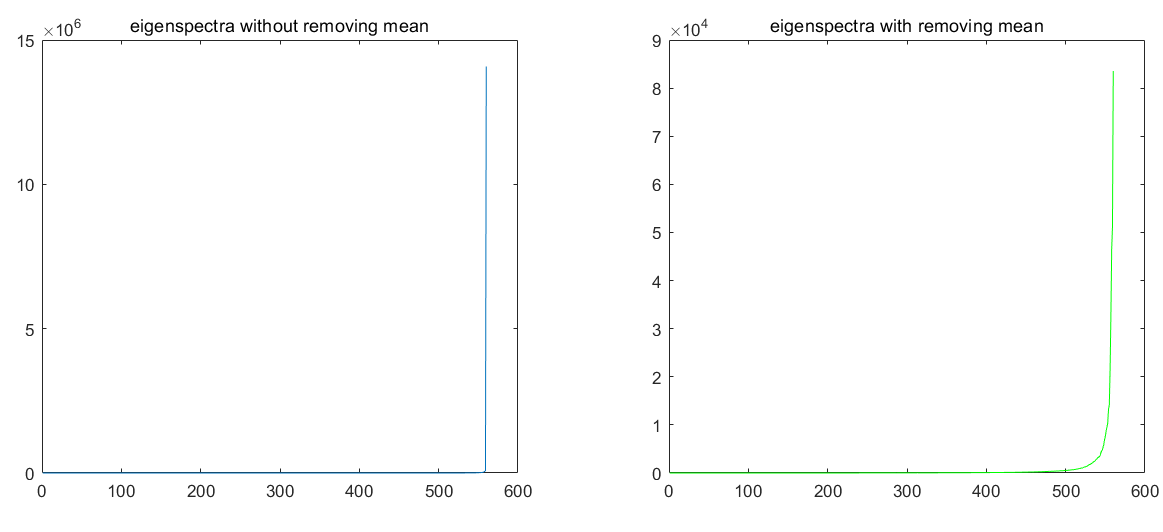
\includegraphics[scale=0.5]{figure10}
	\caption{Left: eigenspectrum of uncentralized $X$. Right: eigenspectrum of centralized $X$.}
	\label{fig10}
\end{figure}

Eigenspectra of the uncentralized and centralized $X$ are in \textbf{Figure \ref{fig10}}. Notice the vertical axis of the two, the eigenvalues of the left are as much as $10^2$ times bigger than the right ones, which verifies my theoretical analysis.

\subsubsection{Chosen of k}
A good choice for $k$ should satisfies the condition that the chosen $k$ principle components reserves most of the information in $X$. That is to say:
\[
\frac{\mathrm{Var}[X\Phi_k]}{\mathrm{Var}[X]}=\frac{\Vert X\Phi_k\Vert_2^2}{\Vert X\Vert_2^2}\ge 1-\varepsilon
\]
where $k$ is the number of chosen principle components (also the number of eigenvectors) and $\varepsilon$ is a hyperparameter which represents for the proportion of abandoned information. We should choose it according to our demand.\par
In practice, the common values of $\varepsilon$ are $5\%$ and $1\%$. Here we set $\varepsilon=5\%$ and get the results below. It suggests we can reduce the dimension of input data from 560 to 80 with only $5\%$ information loss.

\begin{commandline}
	\begin{verbatim}
k = 80 with 0.950536 variance reserved
	\end{verbatim}
\end{commandline}

\subsection{Top 16 eigenvectors}
The facec images of the top 16 eigenvectors are shown in \textbf{Figure \ref{fig11}}. They have some difference as well as some similarities.

\begin{figure}[H]
	\centering
	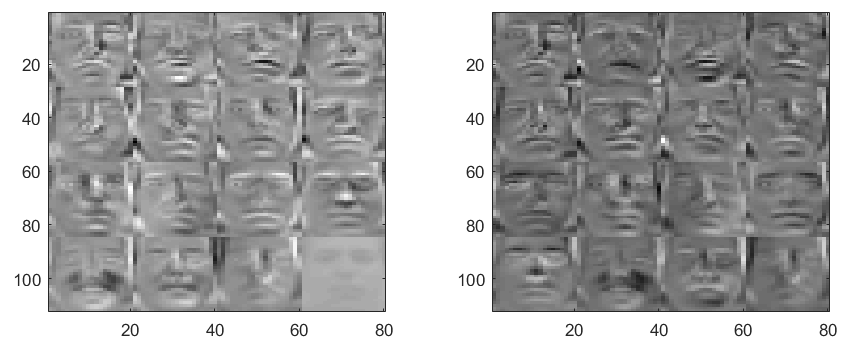
\includegraphics[scale=0.7]{figure11}
	\caption{Left: projected images in uncentralized case. Right: projected images in centralized case.}
	\label{fig11}
\end{figure}

\paragraph{color} The faces on the left are more shallow and bright in color than the right ones. The difference in color is caused by the centralization operation in \textbf{2.1.1}. Centralized data has been subtracted its mean (a positive value), so its eigenvector seems more dark in grayscale pictures where 0 represents black and 255 represents white.

\paragraph{shape} Some of the faces have the same shape, or in other words, the same expressions, such as the first face on the left with the first on the right, the fourth on the left with the fifth on the right. Many eigenvectors of uncentralized $X^TX$ have the same shape as centralized ones, only differ in color and order. It implies that both the eigenvectors of uncentralized and centralized data can capture some common features of the faces.

\paragraph{order} We can find that the order of the faces which have the same shape (or say expression) are different on the two side, despite the fact that all the eigenvectors are sorted by the magnitude of corresponding eigenvalues, while big eigenvalue corresponds to big variance in the combination of input dimensions. So the order of the faces manifests the importance order of the features.\par
But what impressed me most is the last eigenvector that corresponds to the biggest eigenvalue in each side. Just as I analysed in \textbf{2.1.1}, the variance of the first principle component becomes huge in uncentralized case due to an extra term in it. The extra term is the variance of the mean value of each instance, and is about $10^2$ bigger than the variance of the first principle component, completely covering the features of faces. So the last face on the left is so vague and blurred that it provides us with little information about the feature of Brendan Frey’s face. This phenomenon stressed the importance of centralization again.

\subsection{2D points}
When projecting the data onto eigenvectors, the range of the axis is proportional to the variance of the principle components. In \textbf{Figure \ref{fig12}}, the vertical and horizontal axis respectively corresponds to the first and second principle components (abbr PC) of the data. On the left side, the first PC ranges from about 3300 to 4100, and second PC from -600 to 800. On the right, the first PC ranges from -1000 to 500 and second from -400 to 800.\par
The first PC in uncentralized case is not zero-centered and its range are more narrow than its second PC, so contains less information than the second PC, needless to say the first PC in centralized case. Therefore, the second PC in uncentralized case has a wider range and contains more information. This distribution also proved the analysis in \textbf{2.2}.\par
In centralized case, the fist PC has a wider range than the second PC, thus containing more information. Besides, both of them are approximately zero-cetered.\par
This part illustrate the importance of centralization once more.

\begin{figure}[H]
\begin{minipage}[t]{0.5\linewidth}
\centering
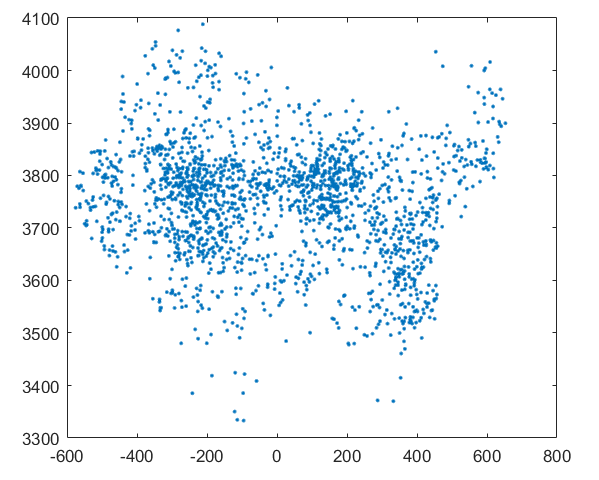
\includegraphics[width=3in]{figure12_1}
\end{minipage}%
\begin{minipage}[t]{0.5\linewidth}
\centering
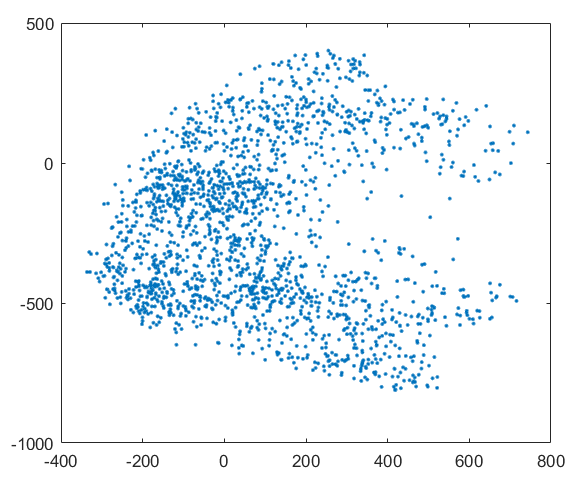
\includegraphics[width=3in]{figure12_2}
\end{minipage}
\caption{Project the data onto the top two eigenvectors. Left: uncentralized. Right: centralized.}
\label{fig12}
\end{figure}

\subsection{Reconstruction}
The problem of reconstruction can be written as a least square problem:
\[
\begin{aligned}
\min_X\Vert V^TX-Y\Vert_2^2\\
\end{aligned}
\]
which can be solved by:
\[
\hat{X}=V^\dagger Y=(V^TV)^{-1}V^TY
\]

Randomly select a $Y$ and corresponding recovered images $\hat{X}$ are shown in \textbf{Figure \ref{fig13}}. It look reasonable since they're similar to the origin image (center) but a little vague, because we have only used two PCs to recover it. And the recovered image in centralized case (right) is more detailed than the uncentralized one (left), especially the nose and mouth.

\begin{figure}[H]
	\centering
	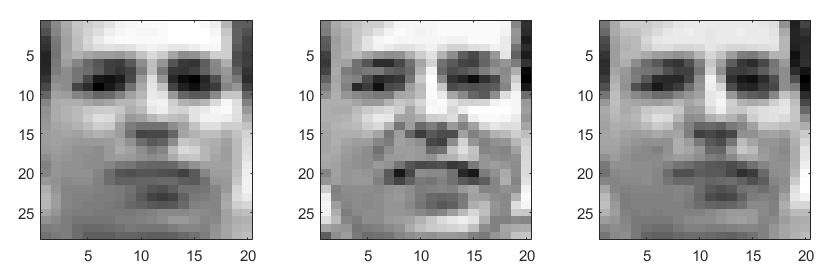
\includegraphics[scale=0.6]{figure13}
	\caption{Recovered image. Left: uncentralized case. Center: origin image. Right: centralized case.}
	\label{fig13}
\end{figure}

\subsection{Reconstruction with noise}
In the case of Gaussian white noise with noise power $P_n=\sigma_n^2=1$. The result is terrible: reconstructed image seems more fuzzy. It demonstrates we should include more PCs in $Y$ to counteract the influence of noise. As I showed in \textbf{2.1.2}, we can choose top 80 eigenvectors in stead of only 2 to reserve as much as $95\%$ information of the image.
\begin{figure}[H]
	\centering
	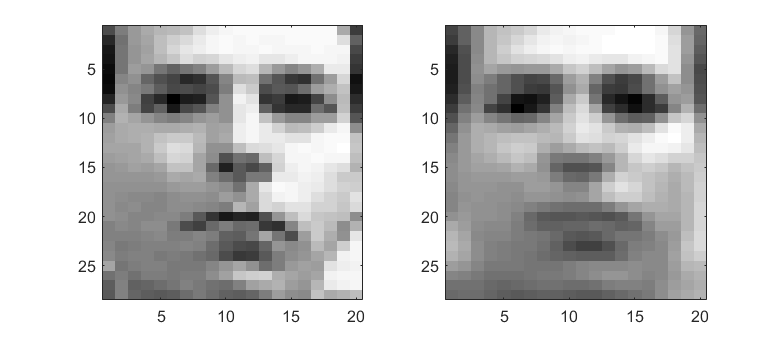
\includegraphics[scale=0.6]{figure14}
	\caption{Reconstruction with noise. Left: origin image. Right: reconstructed image.}
	\label{fig14}
\end{figure}

See codes of \textbf{$2.1\sim 2.5$} in Matlab file $PCA.m$.

\subsection{LLE}
LLE is a method to realize dimensionality reduction based on manifold learning. Different from PCA, LLE concentrate on the local instead of global linearity of the data and use the idea of K-nearest neighbour. It works well with the data which cannot be clustered according to their Euclid distance.

\begin{figure}[H]
	\centering
	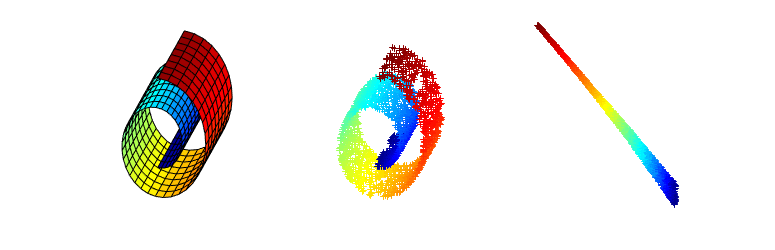
\includegraphics[scale=0.8]{figure15}
	\caption{LLE of swissroll.}
	\label{fig15}
\end{figure}
\pagebreak

\section{Gaussian Mixture Model}

\subsection{EM for Mixture of Gaussians}
Under the condition of $\Sigma_k=\Sigma,\forall k$, the EM equations can be maximized in a simpler manner.

\paragraph{E step}According to Bayes rule, the posterior can be evaluated as:
\[
\begin{aligned}
\gamma(z_k)&=p(z_k=1\mid x)\\
&=\frac{p(z_k=1)p(x\mid z_k=1)}{\sum_{j=1}^Kp(z_j=1)p(x\mid z_j=1)}\\
&=\frac{\pi_k\mathcal N(x\mid \mu_k,\Sigma)}{\sum_{j=1}^K\pi_j\mathcal N(x\mid \mu_j,\Sigma)}\\
&=\frac{\pi_k \exp[(x-\mu_k)^T\Sigma^{-1}(x-\mu_k)]}{\sum_{j=1}^K\pi_j \exp[(x-\mu_j)^T\Sigma^{-1}(x-\mu_j)]}
\end{aligned}
\]
where $k$ is the correct class.

\paragraph{Log-likelihood}
\[
\begin{aligned}
\ln p(X\mid\pi,\mu,\Sigma)&=\sum_{n=1}^N\ln\left(\sum_{k=1}^K\pi_k\mathcal N\left(x^{(n)}\mid\mu_k,\Sigma\right)\right)\\
&=\sum_{n=1}^N\left(
-\frac{1}{2}\ln2\pi\mid\Sigma\mid+\ln\sum_{k=1}^K\pi_k\exp\left(-\frac{1}{2}(x-\mu)^T\Sigma^{-1}(x-\mu)\right)\right)
\end{aligned}
\]

\paragraph{M step}
Let $\frac{\partial\ln p(X\mid\pi,\mu,\Sigma)}{\partial\mu_k}=0$ and $\frac{\partial\ln p(X\mid\pi,\mu,\Sigma)}{\partial\Sigma}=0$ we get
\[
\begin{aligned}
\mu_k&=\frac{1}{N_k}\sum_{n=1}^N\gamma\left(z_k^{(n)}\right)x^{(n)}\\
\Sigma&=\frac{1}{N_k}\sum_{n=1}^N\gamma\left(z_k^{(n)}\right)\left(x^{(n)}-\mu_k\right)\left(x^{(n)}-\mu_k\right)^T\\
\pi_k&=\frac{N_k}{N}
\end{aligned}
\]

where $\gamma\left(z_k^{(n)}\right)$ has been evaluated in E step and $N_k=\sum_{n=1}^N\gamma\left(z_k^{(n)}\right)$.\par

\subsection{Mixtures of Gaussians}
Read codes (see comments in the codes). In the codes, several tricks are used to simplify and accelerate evaluation, such as: subtract the maximum in the vector both on numerator and denominator to avoid overflow when evaluating exponential and $\frac{1}{N_k}=\frac{1}{\pi_kN}$ in M step.

\subsection{Training}
To start with, load data and show random one in grayscale image for both training set (digits 2 and 3) to assure that they are loaded successfully.\par

\begin{figure}[H]
	\centering
	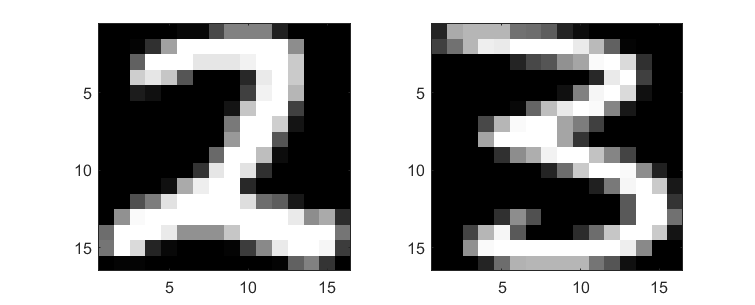
\includegraphics[scale=0.5]{figure16}
	\caption{A random instance in training set for both digits 2 and 3.}
	\label{fig16}
\end{figure}

Then, fix number of clusters $K=2$ and minimum variance $minVar=0.01$ and experiment with parameter settings $randConst$ and iteration times $iters$.

\paragraph{digits 2}
Through experiments to get the largest $\log P(D)$ with iterations needed for convergency as little as possible, the best parameters for digits 2 are $randConst = 10$ and $iters = 10$. Related figures are plot in \textbf{Figure \ref{fig17},\ref{fig18}}.\par
The features of the two clusters are significant in \textbf{Figure \ref{fig18}}. The fist cluster (k=1) represents for the digits which is written starting from the upper left corner and don't include a circle. On the contrary, the second cluster (k=2) represents for the digits that is written starting form the upper middle position and include a circle.\par
These features can also be inferred from \textbf{Figure \ref{fig17}}, where the green ellipse and points corresponds to the first cluster (k=1) and red for the second (k=2). Since the plot only shows the first 2 dimensions of the digits, i.e., two pixels in the upper left corner. The mean of first 2 dimensions for the first cluster is not (0,0) and all of the green points are not located in (0,0) in their first 2 dimensions, which indicates these digits has been written starting from the upper left corner. The situation is the opposite for the second cluster with mean (0,0).\par

\begin{figure}[H]
\begin{minipage}[t]{0.5\linewidth}
\centering
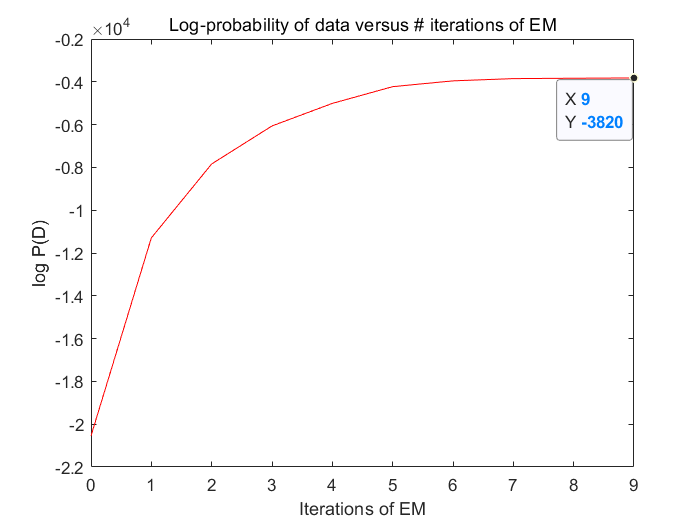
\includegraphics[width=3in]{figure17_1}
\end{minipage}%
\begin{minipage}[t]{0.5\linewidth}
\centering
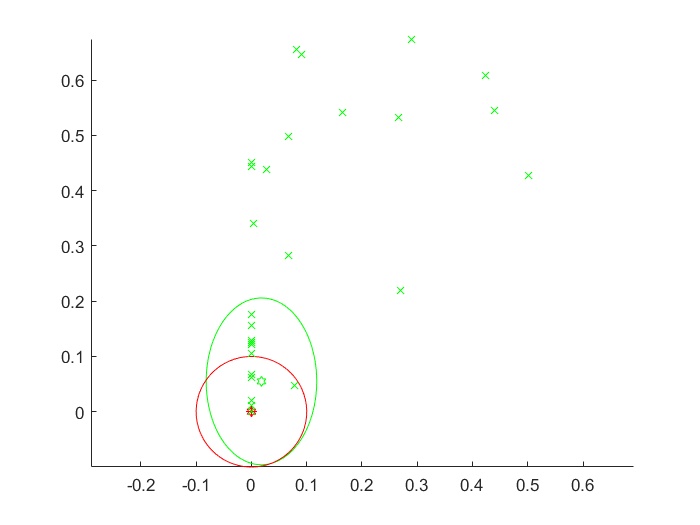
\includegraphics[width=3in]{figure17_2}
\end{minipage}
\caption{$\log P(TrainingData)$ and clusters for the fist two dimensions.}
\label{fig17}
\end{figure}

\begin{figure}[H]
	\centering
	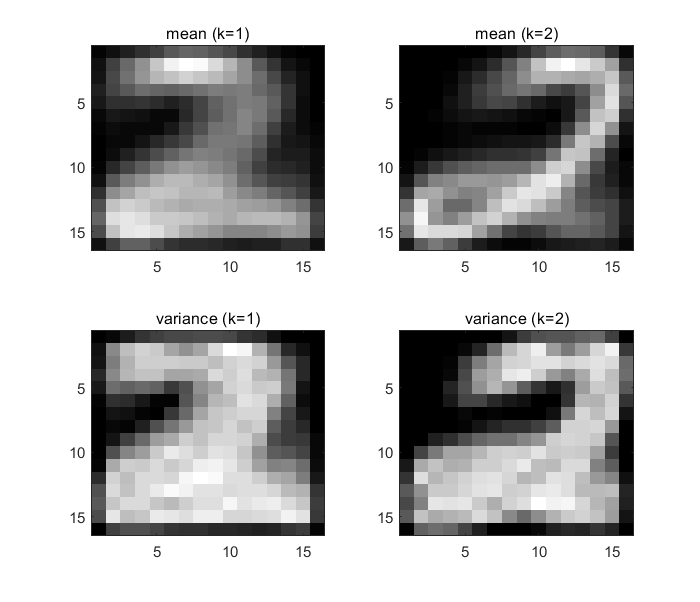
\includegraphics[scale=0.6]{figure18}
	\caption{Mean and variance of two clusters.}
	\label{fig18}
\end{figure}

Results of mixing proportions and final log-likelihood:
\begin{table}[H]
	\centering
	\caption{Results for digits 2.}
	\label{tab5}
	\begin{tabular}{ccc}
	\toprule
	$\pi_1$ & $\pi_2$ & $\log P(TrainingData)$\\
	\midrule
	0.4833 & 0.5167 & -3820\\
	\bottomrule
	\end{tabular}
\end{table}

\paragraph{digits 3}
Similarly to digits 2. Through experiments, best parameters are $randConst = 10$ and $iters = 20$. Related figures are shown in \textbf{Figure \ref{fig19},\ref{fig20}}.\par
The features for 2 clusters in digits 3 are also marked. Digits in the fist cluster normal and start from the upper left corner (corresponds to the green ellipse and points), while digits in the second cluster are tilted and starts from the upper middle position (corresponds to the red ellipse and points).\par

\begin{figure}[H]
\begin{minipage}[t]{0.5\linewidth}
\centering
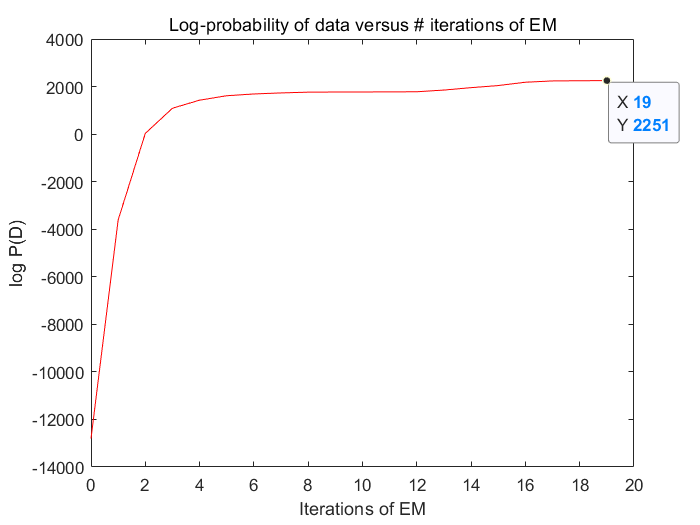
\includegraphics[width=3in]{figure19_1}
\end{minipage}%
\begin{minipage}[t]{0.5\linewidth}
\centering
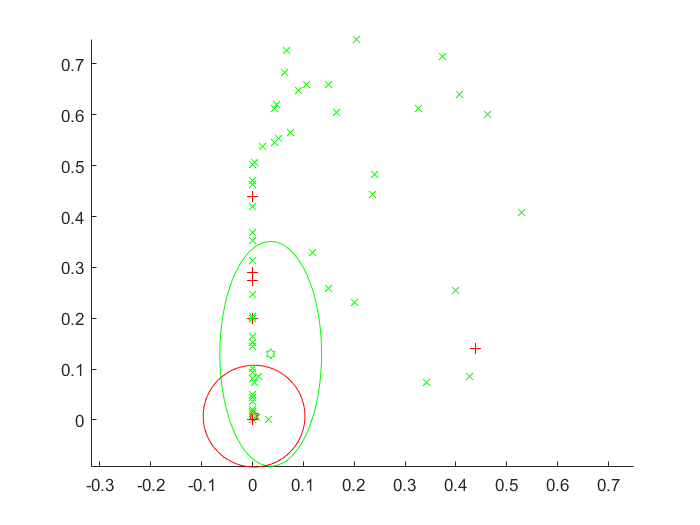
\includegraphics[width=3in]{figure19_2}
\end{minipage}
\caption{$\log P(TrainingData)$ and clusters for the fist two dimensions.}
\label{fig19}
\end{figure}

\begin{figure}[H]
	\centering
	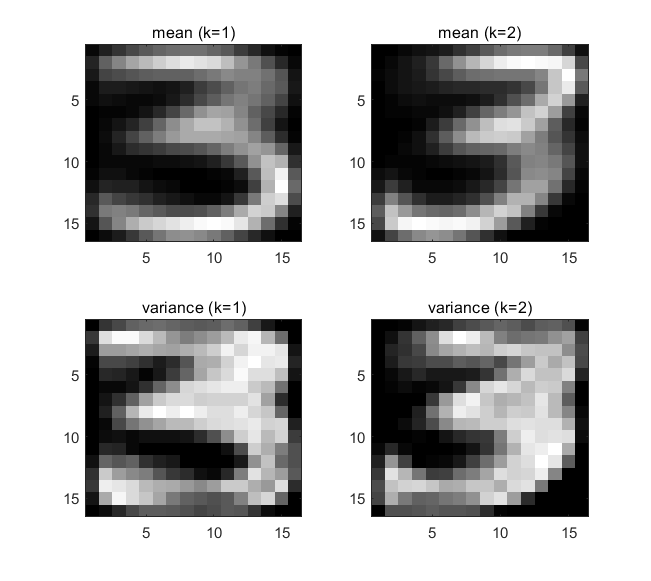
\includegraphics[scale=0.6]{figure20}
	\caption{Mean and variance of two clusters.}
	\label{fig20}
\end{figure}

Results of mixing proportions and final log-likelihood:
\begin{table}[H]
	\centering
	\caption{Results for digits 3.}
	\label{tab6}
	\begin{tabular}{ccc}
	\toprule
	$\pi_1$ & $\pi_2$ & $\log P(TrainingData)$\\
	\midrule
	0.5061 & 0.4939 & 2251\\
	\bottomrule
	\end{tabular}
\end{table}
See codes of \textbf{3.3} in \textit{run\_q1}

\subsection{Initializing a mixture of Gaussians with k-means}
\paragraph{\textit{kmeans.m and distmat.m}}
I made a trivial improvement during the evaluation process of \textit{kmeans} based on provided code to accelerate evaluation: just replace the first \textit{for} loop in it with \textit{dist = distmat(means', x');}.

\paragraph{\textit{mogEM.m}}
When initializing $\mu$, choose whether to use \textit{kmeans} according to the 6th input argument \textit{Kmeans}.
\begin{lstlisting}
if nargin==6 && Kmeans
    mu = kmeans(x, K, iters);
else
    mn = mean(x,2);
    mu = mn*ones(1,K)+randn(N,K).*(sqrt(vr)/randConst*ones(1,K));
end
\end{lstlisting}

\paragraph{Train MoG models}
Set number of components $K=20$ and concatenate 600 training vectors (both 2’s and 3’s). Then, use original initialization and the one based on k-means perspectively. Results are plotted in \textbf{Figure \ref{fig21},\ref{fig22}}.\par
When training with original initialization, it takes about 20 iterations to converge with $logP(D)=2.681\times 10^{4}$,while training with kmeans initialization only requires 10 times and results in a higher log-probability of $logP(D)=2.904\times 10^{4}$.\par

\begin{figure}[H]
\begin{minipage}[t]{0.5\linewidth}
\centering
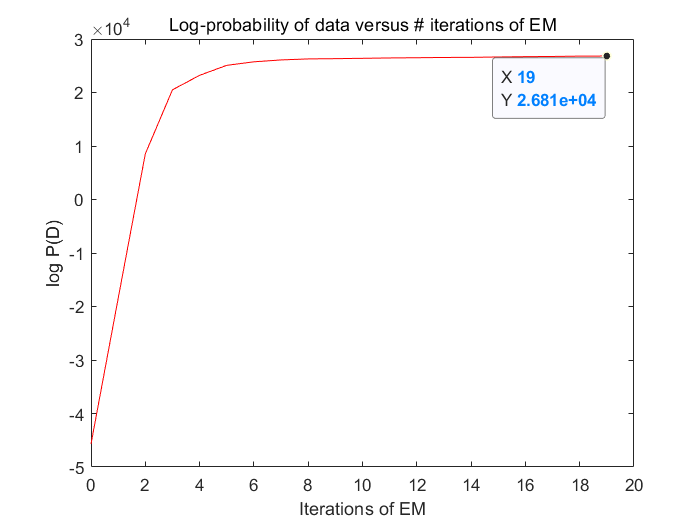
\includegraphics[width=3in]{figure21_1}
\end{minipage}%
\begin{minipage}[t]{0.5\linewidth}
\centering
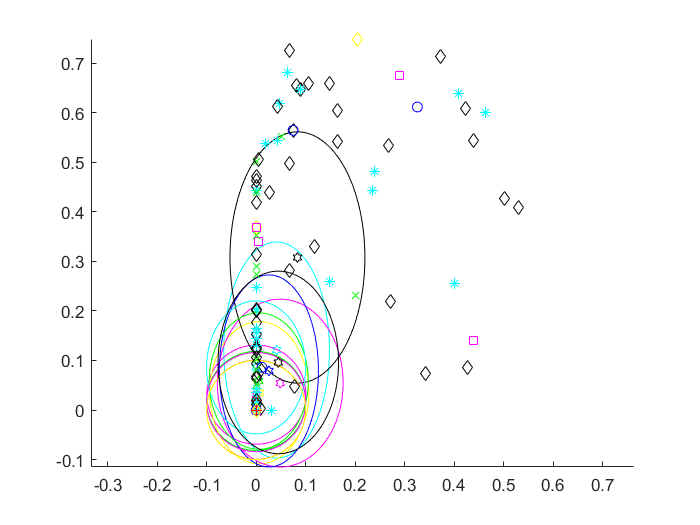
\includegraphics[width=3in]{figure21_2}
\end{minipage}
\caption{Train with original initialization.}
\label{fig21}
\end{figure}

\begin{figure}[H]
\begin{minipage}[t]{0.5\linewidth}
\centering
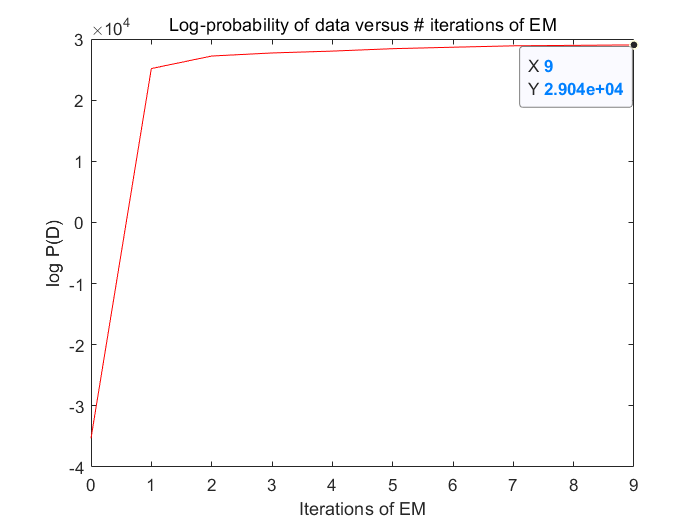
\includegraphics[width=3in]{figure22_1}
\end{minipage}%
\begin{minipage}[t]{0.5\linewidth}
\centering
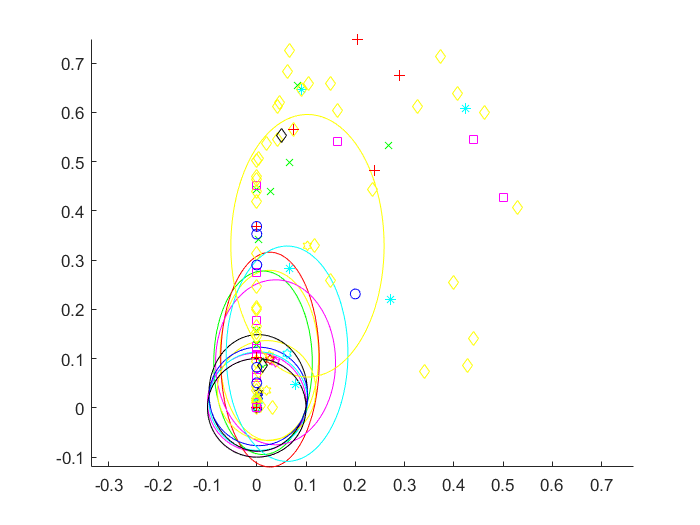
\includegraphics[width=3in]{figure22_2}
\end{minipage}
\caption{Train with kmeans initialization.}
\label{fig22}
\end{figure}
See codes in \textit{run\_q3.m}.

\subsection{Classification using MoGs}
Use \textit{mogLogProb.m} to calculate the log-probability of the input set on the two models perspectively, and let the model that has the largest log-probability be the predicted class, then compare with true and compute error rate. In the code, I have fix the parameters $iters=20$ and $minVar=0.01$ to make sure each model with every component could converge.Results are in \textbf{Figure \ref{fig23}}. See codes in \textit{run\_q4.m}.\par


\paragraph{Answer to the questions on the paper:}\quad\par
\textbf{1.} In fact, components plays as a role to recognize patterns of the image, just as we have seen in \textbf{Figure \ref{fig18},\ref{fig20}}, different means of clusters show different patterns. So when we increase the number of components, we can get more patterns of the images, and the correct class with more correct pattern may generate a higher log-probability score than the false class. Therefore, we can distinguish different classes according to different patterns they have.\par

\textbf{2.} With the increasing of components, the test error declines firstly and then rises up a little (from 15 to 25), and it's the same to the test error, which implies overfitting occurred when we increase it too much.\par

\textbf{3.} I'd like to select the model with 15 components, since it has the lowest test error. There also exists a bias-variance trade-off. When we increase the number of components, bias gets lower while variance gets higher, so we should only increase it appropriately to make sure overfitting hasn't occurred. The model with the lowest test error has the best ability of generalization, thus performing best on new images.

\begin{figure}[H]
	\centering
	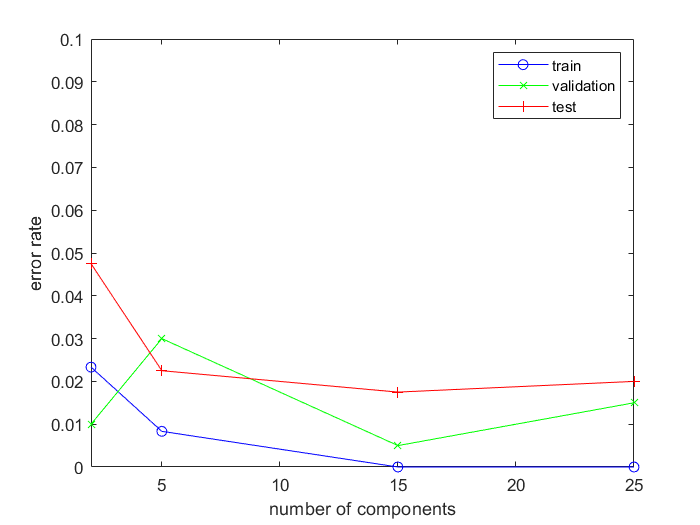
\includegraphics[scale=0.6]{figure23}
	\caption{Error rate for different number of components.}
	\label{fig23}
\end{figure}

\end{document}
